%; whizzy chapter
% -initex iniptex -latex platex -format platex -bibtex jbibtex -fmt fmt
% 以上 whizzytex を使用する場合の設定。

%     Kansai Debian Meeting resources
%     Copyright (C) 2007 Takaya Yamashita
%     Thank you for Tokyo Debian Meeting resources

%     This program is free software; you can redistribute it and/or modify
%     it under the terms of the GNU General Public License as published by
%     the Free Software Foundation; either version 2 of the License, or
%     (at your option) any later version.

%     This program is distributed in the hope that it will be useful,
%     but WITHOUT ANY WARRANTY; without even the implied warranty of
%     MERCHANTABILITY or FITNESS FOR A PARTICULAR PURPOSE.  See the
%     GNU General Public License for more details.

%     You should have received a copy of the GNU General Public License
%     along with this program; if not, write to the Free Software
%     Foundation, Inc., 51 Franklin St, Fifth Floor, Boston, MA  02110-1301 USA

%  preview (shell-command (concat "evince " (replace-regexp-in-string "tex$" "pdf"(buffer-file-name)) "&"))
% 画像ファイルを処理するためにはebbを利用してboundingboxを作成。
%(shell-command "cd image200708; ebb *.png")

%%ここからヘッダ開始。

\documentclass[mingoth,a4paper]{jsarticle}
\usepackage{kansaimonthlyreport}
\usepackage{ascmac}

% 日付を定義する、毎月変わります。
\newcommand{\debmtgyear}{2008}
\newcommand{\debmtgdate}{29}
\newcommand{\debmtgmonth}{6}
\newcommand{\debmtgnumber}{14}

\begin{document}

\begin{titlepage}

% 毎月変更する部分, 本文の末尾も修正することをわすれずに

 第\debmtgnumber{}回 関西 Debian 勉強会資料

\vspace{2cm}

\begin{center}
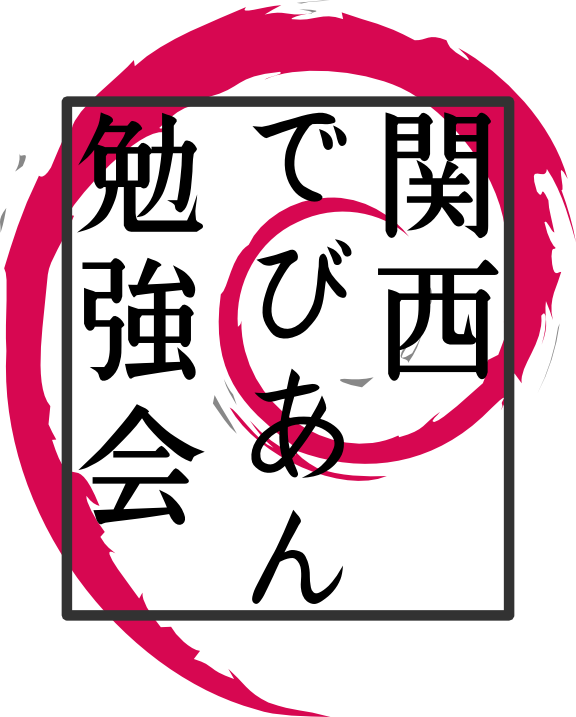
\includegraphics{image200802/kansaidebianlogo.png}
\end{center}

\begin{flushright}
\hfill{}関西 Debian 勉強会担当者 山下 尊也\\
\hfill{}\debmtgyear{}年\debmtgmonth{}月\debmtgdate{}日
\end{flushright}

\thispagestyle{empty}
\end{titlepage}

\dancersection{Introduction}{山下 尊也}
 
 関西 Debian 勉強会はDebian GNU/Linux のさまざ
 まなトピック(新しいパッケージ、Debian 特有の機能の仕組、Debian 界隈で起
 こった出来事、などなど)について話し合う会です。

 目的として次の三つを考えています。
 \begin{itemize}
  \item MLや掲示板ではなく、直接顔を合わせる事での情報交換の促進
  \item 定期的に集まれる場所
  \item 資料の作成
 \end{itemize}

 それでは、楽しい一時をお楽しみ下さい。

\newpage

\begin{minipage}[b]{0.2\hsize}
 {\rotatebox{90}{\fontsize{80}{80}
{\gt 関西デビアン勉強会}}}
\end{minipage}
\begin{minipage}[b]{0.8\hsize}
\hrule
\vspace{2mm}
\hrule
\setcounter{tocdepth}{1}
\tableofcontents
\vspace{2mm}
\hrule
\end{minipage}

\dancersection{最近のDebian関係のイベント報告}{山下 尊也}
\subsection{第13回 関西 Debian 勉強会}
2008年5月18日に「第13回 関西 Debian 勉強会」を行いました。
勉強会は、合計25名の参加でした。

\subsubsection{発表内容}

\begin{itemize}
 \item ustream.tvを使った関西Debian勉強会中継の裏側
 \item Debianで始めるEmacsエディタ
 \item 自宅LANでIPv6のルータを作ってみよう(Part1)
\end{itemize}

姫路で行われた第12回 関西 Debian 勉強会では、
ustream.tv を使った関西Debian勉強会中継の裏側
と言う事でお話して頂きました。
「ストリーミング中継で何を重視するのか?」や
実際に、「たかやが失敗したポイント」などをまとめて頂きました。
また、関西 Debian 勉強会では、今後も ustream.tv を使った中継を考えていま
す。

Debianで始める Emacsと言うことで、木下さんに講師をして頂きました。
普段から Emacs を使っている人は、Debianユーザには多いと思いますが、
知らなかったことなどもあったのではないかと考えています。

IPv6のルータを作ろうと言うことで、川江さんに講師をして頂きました。
また、勉強会には東京から吉藤さんも来ており、IPv6の入門者向け資料が
不足しているとの事で、川江さんが今後、IPv6について調査し、まとめて頂くと
の事です\verb|:)|

\dancersection{pbuilder でパッケージをビルドしてみる}{大浦 真}

\subsection{pbuilder とは}

\begin{itemize}
\item 現在稼働中のシステムの中に新しい chroot 環境を作り
  その中でパッケージをビルドするためのシステム。
  \begin{itemize}
  \item chroot: ルートディレクトリを変更してコマンドを実行するための
    コマンド。
    現在稼働しているものとは別のディレクトリツリーを用意し、
    そこで、さまざまなテストを行うことができる。
    実機や仮想マシンは必要ない。
  \end{itemize}
\item Debian パッケージはビルド環境の状態によって、
  ビルドできなくなることもある。
\item pbuilder を使って、パッケージがまっさらな環境できちんとビルドできるか
  確認できる。
\item pbuilder は base システムだけの chroot 環境を用意してくれるので、
  パッケージの Build-Depends: フィールドが正しいかチェックできる。
\end{itemize}


\subsection{pbuider の使い方}

\begin{itemize}
\item pbuilder のインストール。
\item 設定ファイルのチェック (/etc/pbuilderrc)。
\item \texttt{pbuilder} コマンドの実行には root 権限が必要になる。
\item \texttt{pbuilder create} で最新の base システムだけの chroot 環境を
  作成する。
  その chroot 環境を tar+gzip でまとめたものが
  \texttt{/var/cache/pbuilder/base.tgz} に作成される。
\item \texttt{pbuilder update} で chroot 環境を更新する。
\item \texttt{pbuilder build \underline{package}.dsc} として
  .dsc ファイルを指定し、chroot 環境内でビルドを行う。
  \begin{itemize}
  \item ビルド環境の設定などに依存せずにビルドできるか確認できる。
  \item Build-Depends: に指定されているパッケージは自動的に
    インストールされるので、足りないパッケージがないか確認できる。
  \end{itemize}
\item ビルドされたパッケージは \texttt{/var/cache/pbuilder/result} に置かれる。
\item ビルドの途中でダウンロードされたパッケージは、
  \texttt{/var/cache/pbuilder/aptcache} に置かれる。
  このディレクトリのファイルは \texttt{pbuilder clean} で削除される。
\item \texttt{pbuilder login} で、chroot 環境の中の shell に入ることができる。
\end{itemize}


\subsection{cowdancer と cowbuilder}

\begin{itemize}
\item pbuilder は base.tgz の展開に時間がかかるという欠点がある。
\item cowdancer はファイルシステムの Copy-on-Write を提供する。
  \begin{itemize}
  \item ディレクトリ構造をハードリンクでコピーしておき、
    実際に書き込みがあった時にハードリンクの関係を解消してくれる。
  \end{itemize}
\item cowbuilder は base.tgz を展開する代わりに、展開済のベースシステムを
  ハードリンクでコピーして利用してくれる。
\end{itemize}

\subsection{関連コマンド・パッケージ}

\begin{itemize}
\item \texttt{pdebuild}: pbuilder パッケージに含まれている。
  \texttt{debuild} のように Debian パッケージのソースツリーの中で使う。
  \texttt{cowbuilder} を使う時は、\texttt{pdebuild --pbuilder cowbuilder}と
  する。
\item pbuilder-uml (User Mode Linux) を使うと pbuilder の実行に
  root 権限は不要になる(らしい)。
\end{itemize}

\subsection{参考 URL}

\begin{itemize}
\item \url{http://tokyodebian.alioth.debian.org/2006-06.html} \\
  第17回東京エリアDebian勉強会 事前配布資料
\item \url{http://www.netfort.gr.jp/~dancer/software/pbuilder-doc/pbuilder-doc.html} \\
  pbuilder User's Manual
\item \url{http://www.netfort.gr.jp/~dancer/software/pbuilder.html} \\
  pbuilder - Personal builder
\item \url{http://www.netfort.gr.jp/~dancer/software/cowdancer.html} \\
  cowdancer - copy-on-write data access completely in userland
\end{itemize}

\dancersection{SSL のサーバー証明書が失効する時}{久保 博}

Debian Project\index{Debian Project} から発表された Debian セキュリティ
勧告の DSA--1571 は、 OpenSSL\index{OpenSSL} の脆弱性に関するものでした。
この勧告に端を発っした脆弱性の問題は、他の Debian セキュリティ勧告とはや
や異なる波紋を社会に投げかけ、遂には日本べサイン社がプレスリリースを発表
するまで社会的影響が広がりました。
これを機会に、OpenSSL とサーバー証明書について、ユーザーの視点で仕組みを
解説します。

\subsection{最初の経緯}
2008年5月14日「Debian セキュリティ勧告」に、OpenSSL\index{OpenSSL} の脆弱性情報が発表されました。



\begin{description}
\item{DSA-1571-1 openssl -- 予測可能な乱数の生成}\cite{DSA-1571}
\par
\begin{quotation}
Debian システムで、バージョン 0.9.8c-1 以降の OpenSSL で作成された、暗号鍵に関するデータは捨てて作り直す必要があります。さらに、影響を受ける Debian システムで、署名や本人認証の目的で使われた全ての DSA 鍵は脆弱であると考えてください。デジタル署名アルゴリズムは、署名生成時の秘密の乱数の値に依存しているからです。
\end{quotation}

\end{description}

これにより、脆弱性を抱えた OpenSSL を使って生成された電子署名\index{でんししょめい@電子署名}
の鍵は、脆弱であるものと認識され、それには SSL で利用される
X.509\index{X.509} のサーバー証明書も含まれていました。

\subsection{社会的影響}

複数の商用のX.509証明書の認証局から、DSA-1571 のためのサーバー証明書再発行について、声明が発表されました。

%\begin{itemize}
 \paragraph{5月16日 日本クロストラスト}  Debianに含まれるOpenSSLの脆弱性への対応に関するお知らせ\footnote{http://crosstrust.co.jp/company/information/i20080516} 。

   \paragraph{5月19日 サイバートラスト} サーバー証明書の再発行が無料であることをアピール。\footnote{http://www.cybertrust.ne.jp/info/2008/080519.html} 

  \paragraph{5月20日 日本ベリサイン} 「日本ベリサイン、Linux OSの脆弱性による影響を受けたお客様に、電子証明書を再発行」\footnote{http://www.verisign.co.jp/press/2008/pr\_20080520.html}。

  \paragraph{5月21日 Comodo } COMODO OFFERS FREE REPLACEMENT CERTIFICATE TO ANY INDIVIDUALS AFFECTED BY DEBIAN VULNERABILITY FLAW\footnote{http://www.comodo.com/news/press\_releases/21\_05\_08.html}.
  
   \paragraph{5月22日 グローバルサイン} 脆弱性について注意喚起した上で、サーバー証明書の再発行がもともと無料であることさりげなくアピール\footnote{http://jp.globalsign.com/info/report/2008/05/id112} 。
%\end{itemize}

\subsection{サーバー証明書}

まずは、OpenSSLとベリサインなどの認証局との関係を解き明かす為、まず、サーバー証明書について解説します。

\subsubsection{電子署名と電子証明書}

電子署名\index{でんししょめい@電子署名}とは、電子情報に対して付加する特殊な情報です。
電子署名が拠り所とする重要な技術に、「公開鍵暗号\index{こうかいかぎあんごう@公開鍵暗号}」があり、暗号化する鍵と復号する鍵が別々で、しかも、片方は一般に公開しても構わないようにできています。
電子署名を施す署名者 $A$ さんは、秘密の情報 $S_A$ (秘密鍵\index{ひみつかぎ@秘密鍵}) と公開情報 $P_A$ (公開鍵\index{こうかいかぎ@公開鍵})を用意します。
また、署名されるデジタル情報を $M$ としておきます。
\begin{quotation}
$A$ さんが $A$ さんにしか作れないモノを作れば、$A$ さんが確かに $A$ さんであることを示せます。
\end{quotation}

\begin{center}
  \mbox{}\par
\begin{picture}(80,12)(0,0)
%%  \put(0,0){\dashbox{0.5}(80,20){ }}
  \thicklines
  \put(0,10){\line(4,-1){40}}
  \put(40,0){\line(4,1){40}}
  \put(20,5){\line(0,1){20}}
  \put(60,5){\line(0,1){20}}
\end{picture}
\end{center}

\begin{quotation}
$A$ さんしか知らない $S_A$ を使って、電子署名を施すと、署名をした人が確かに $A$ さんであることが示せます。
なお、$A$ さん以外の人がそれを確認するには、 $P_A$ を使います。
\end{quotation}

\begin{center}
  \mbox{}\par
\begin{picture}(80,12)(0,0)
%%  \put(0,0){\dashbox{0.5}(80,20){ }}
  \thicklines
  \put(0,10){\line(4,-1){40}}
  \put(40,0){\line(4,1){40}}
  \put(20,5){\line(0,1){20}}
  \put(60,5){\line(0,1){20}}
\end{picture}
\end{center}

\begin{quotation}
$A$ さんがあることを表明しました。その表明文に $A$ さんしか知らない $S_A$ を使って、電子署名を施すと、確かに $A$ さんがそれを表明したことが示せます。
なお、$A$ さん以外の人がそれを確認するには、 $P_A$ を使います。
\end{quotation}

$M$ の電子署名 $\sigma$ を与える関数を $f$ とすると、

\begin{equation}\label{defsignature}
\sigma = f_{S_A}(M)
\end{equation}

電子証明書は、このように構成されます。簡潔にまとめると、電子証明書の概念上の構成要素は 

\begin{itemize}
\item デジタル情報の形で表された述語
\item 電子署名
\end{itemize}
です。

\subsubsection{公開鍵証明書}

$X$ さんの公開鍵 $P_X$ が、確かに $X$ さんのものであることを表明する電子文書が公開鍵証明書\index{こうかいかぎしょうめいしょ@公開鍵証明書}です。
「$P_X$ が、確かに $X$ さんのものである」という叙述を $m_X$ とすると、
認証局\index{にんしょうきょく@認証局} $C$ がその文書を発行する場合は、式(\ref{defsignature})の $M$ に $P_X$ と $m_X$ の組 $(P_X, m_X)$を、 $S_A$ に $S_C$ を代入したものになります。

\begin{equation}\label{pubkeysignature}
\sigma_X = f_{S_C}((P_X, m_X))
\end{equation}

こうして、ある公開鍵で別の公開鍵を署名する、という関係が生まれました。
これは連鎖させることができます。矢印 $\longrightarrow$ で電子署名する関係を表すと、
\begin{equation}\label{signaturechain}
P_C \longrightarrow P_1 \longrightarrow P_2 \longrightarrow P_3 \longrightarrow P_4 \longrightarrow \cdots
\end{equation}
のような関係を持たせることができるわけです。
$P_C$ は、認証局の公開鍵で、予め信頼できると分かっているものとすれば、
$P_1, P_2, P_3, P_4, \ldots$ はすべて信頼できることになります。

実用上は、単に「公開鍵 $P_A$ が $A$ さんに属する」ということだけでなく、他の述語も一緒に署名されます。
例えば、「$B$ という会社は、実在する会社で、住所はXXXです。」のような表明です。


\subsubsection{ITU-T X.509}
世の中で広く使われている公開鍵の証明書のひとつは、X.509\index{X.509} と言う規格に従ったものです\footnote{最近、これに関係する RFCが発行されました\cite{RFC5280}。}。
もともと、国連の下位機関である国際電気通信連合\index{こくさいでんきつうしんれんごう@国際電気通信連合} (ITU)が定めた勧告です。
その中で、頭に X が付く勧告は、「Xシリーズ勧告」の呼ばれていて、データ通信網に関する勧告が分類されています\footnote{他にもモデムでお馴染みの V.34 や V.90 などの勧告を含む V シリーズなどは馴染み深いでしょう。}。
X.509 では、X.500\index{X.500} 識別名 を利用した公開鍵証明書を定めています\footnote{
X.500 は、ITU-Tが定めたネットワーク上での分散ディレクトリサービスに関する規格で、
\url{http://www.ipa.go.jp/security/fy10/contents/over-all/02/21.html} に詳しいです。}。

ディレクトリサービス\index{ディレクトリサービス}と言うのは、階層的な名前から、それに対応するオブジェクトとその属性とを記憶し、検索できるようにしたシステムです。
「階層的な名前」というものの例を挙げてみると、
\newcounter{ex}
\begin{list}{例\arabic{ex}: }{\protect\usecounter{ex}}
\item 住所と氏名\label{expostaladdress}
\item ファイルシステムのディレクトリとファイル名
\item DNS のドメイン名とホスト名
\end{list}
のようものです。
X.500 では、例\ref{expostaladdress} のような階層的な名前をうまく扱えるようになっていて、
京都府向日市の仮想八百屋さんである八百竹は、X.500風に書くと、
\begin{quote}
C={\em JP}, ST={\em Kyoto}, L={\em Mukou}, CN={\em Yaotake}
\end{quote}
になります。
%% なお、LDAP だとドメイン名を良く使うが、長岡京市のドメイン名が {\tt city.nagaokakyo.kyoto.jp} であることを使って
%% \begin{quote}
%% dc=jp, dc=kyoto, dc=nagaokakyo, dc=city, CN=Yaotake
%% \end{quote}
%% のようにおそらく命名されます。

\subsubsection{SSL のサーバー証明書}
SSL\index{SSL} およびその後継の TLS\index{TLS}\cite{RFC2818}では、通信の最初のハンドシェイクでX.509 の公開鍵証明書\index{こうかいかぎしょうめいしょ@公開鍵証明書}を交換します。
そのうちサーバーからクライアントへ向けて送信される SSL のサーバー証明書は、
クライアント(ブラウザ)から見て、相手のサーバーが確かに自分がアクセスしようとしているサーバーなのかどうかを確認する根拠を提供するのが一つの役目です。
そのために、サーバー証明書には次の情報が含まれています。
\begin{itemize}
\item CN\index{CN} という属性にサーバーの FQDN\index{FQDN} (Fully Qualified Domain Name 完全修飾ドメイン名) を書きます。
\item そのサイトを運営する組織の属性として、 O (組織名), OU (部門),L (住所),ST (都道府県),C (国) を記述します。
\end{itemize}
これらの情報は、認証局にサーバー証明書の発行を依頼する際にサーバー運営者が認証局に提出する証明書署名要求\index{しょうめいしょしょめいようきゅう@証明書署名要求} (Certificate Signing Request 略して CSR\index{CSR}) に最初に記述します。
なお、各認証局毎に細かい差異があります\footnote{例えば TrustCenter GmbH では ST でなくSP. (\tt http://www.trustcenter.de/about/repository.htm)}。
詳しくは、各認証局の CPS\index{CPS} (Certification Practice Statement) やCP\index{CP} (Certificate Policy) という公開された文書に書いてあることもあります。

また、サーバー証明書に含まれる公開鍵が署名だけでなく暗号化にも使える場合は、 SSL のセッション鍵を交換する為にも使われます。

\subsubsection{失効リスト}\label{sec:crl}

公開鍵証明書に含まれている公開鍵が暗号学的に有効であるためには、
\newcounter{cond}
\begin{list}{条件\arabic{cond}. }{\protect\usecounter{cond}}
\item 暗号アルゴリズム的に安全である
\item 秘密鍵が秘密のまま保管されている\label{cond:secret}
\item 鍵の組が十分広い鍵空間から選ばれていて、総当たり攻撃では秘密鍵を推
      定できそうにない\label{cond:broadenough}
\end{list}
が揃っている必要がありますが、時には証明書発行後に、これらの条件が破れて
しまうこともあります。

X.509 を中心とした PKI\index{PKI} (Public Key Infrastructure) の設計では、
このような事態も想定されてます。
ですので、必ず証明書には有効期限が定められていて、時代遅れの証明書がいつ
までも出回らないようにしています。

また、もしも、これらの条件を満たさなくなった「もう使えない」証明書が発生
したら、認証局\index{にんしょうきょく@認証局}にその旨を申し出ます。
すると、認証局は、その証明書を「失効リスト\index{しっこうりすと@失効リスト}(Certificate
Revocation List 略して CRL\index{CRL})」に掲載します。
CRL\index{CRL} は、認証局が配布していて、どこで手に入れたら良いかは、公
開鍵証明書の中に予め、cRLDistributionPoints という属性で示してあります。
最近目にする証明書では、ほとんどの場合 http で始まる URL が書かれていま
すが、サーバー証明書の設計上は LDAP\index{LDAP} のディレクトリサーバーで
配布することも想定されているようです。

なお、CRL\index{CRL} に掲載されるのは、失効した証明書の Serial
Number\index{Serial Number} という属性値と失効した日付です。
CN\index{CN} (即ち、サーバー証明書のホスト名)は載っていませんので、どの
サーバーの証明書が失効したかは、CRL を見ただけでは分かりません。

\subsection{サーバー証明書の失効}
\subsubsection{DSA--1571 の OpenSSL の脆弱性と公開鍵の関係}

SSL のサーバーを構築する上で OpenSSL\index{OpenSSL} のパッケージが関係す
る処理をざっと挙げると
\begin{enumerate}
\item 鍵の組の生成
\item 証明書署名要求 (Certificate Signing Request あるいは略して
      CSR\index{CSR}) の生成
\item web サーバーの SSL の暗号通信の処理。 Apache httpd の mod\_ssl な
      ど。
\end{enumerate}
があります。
DSA--1571 は、乱数の質が悪く、鍵の組の生成で容易に推定できる範囲でしか乱
数を生成していなかった、ということが問題になっていましたので、
\ref{sec:crl}節の条件\ref{cond:broadenough} が満たされなくなった、と言う
のが DSA--1571 から発生した問題です。

\subsubsection{秘密鍵が暴かれることで成り立つ攻撃}
サーバー証明書の秘密鍵が暴かれることことで成立する攻撃には、次のようなも
のが考えられます。
\begin{enumerate}
\item SSL 通信の Man-in-the-middle 攻撃\index{Man-in-the-middle こうげき@Man-in-the-middle 攻
      撃}\label{enum:man-in-the-middle}
\item SSL 通信のパケットを盗聴して記録しておき、後からSSL のハンドシェイ
      クを破り、秘密の通信内容を暴く\label{enum:sniff}
%% \item サーバー証明書を使った公開鍵認証のバイパス\label{enum:pubkeyauth}
\item コンピューターウィルス\index{コンピューターウィルス}を使った hosts
      ファイルへの贋サーバーの登録や DNS cache poisoning\index{DNS cache
      poisoning} と組み合わせて、贋の SSL サーバーを立てる\footnote{つま
      り、例えばフィッシング詐欺\index{ふぃっしんぐさぎ@フィッシング詐欺}を仕掛けるわけで
      す。}\label{enum:phishing}
\end{enumerate}

\ref{enum:man-in-the-middle},  \ref{enum:sniff} は、安全な公開鍵に変更す
れば、変更後は安全になります。

\ref{enum:phishing} に関しては、サーバー管理者が脆弱な公開鍵を SSL で使
うことを止め、安全な公開鍵に交換したとしても、
公開鍵を変更する前に脆弱な公開鍵を攻撃者が入手していれば、成立します。
但し、サーバー管理者が認証局に申請して脆弱な公開鍵を失効させてくれれば、
脆弱な公開鍵が CRL\index{CRL} に掲載されます。
ほぼすべての認証局は、CPS\index{CPS} などで失効手続きについて規定してお
り、失効申請の窓口も完備しているはずですので、
サーバー管理者さえしっかりしていてくれれば、脆弱な公開鍵を失効はしてもら
えます。
ですので、あとは、クライアント側が CRL を入手できれば、
\ref{enum:phishing} の攻撃を回避することもできるわけです。

クライアントの立場でSSL のサーバーを利用する場合、すなわち、https で始ま
る URL のサイトに訪問する場合には、
\ref{sec:rpa}節で説明する事項に合意の上、なるべく新しい CRL を入手し、お
手元のブラウザに取り込みましょう。

すると、ブラウザが CRL と照合してサーバー証明書の有効性を確認してくれま
す。

\subsubsection{証明書の失効リストを取り込む方法}

現在は、認証局は CRL を web サーバーで提供することが多いです。
ですので、配布元の URL が分かれば web ブラウザで取得することができます。

また、Iceweasel\index{Iceweasel}\footnote{もちろん、 Mozilla FireFox も、
です。} は、CRL の URL へアクセスすると、
自動的にローカルで管理している失効リストに追加しようとします%
%\footnote{MIME type が application/x-pkcs7-crl のエンティエティを CRL として扱います。}
。

\subsubsection{Iceweasel で表示した SSL のページの CRL を取得する}

SSL のページにアクセスして、表示されたページの上で右クリックすると、メ
ニューが表示されます。
ここで[ページの情報の表示]を選択し、[セキュリティ] タブを選択し、[表示]
を選択します。
すると、別窓に証明書ビューアが立ち上がります。ここで [詳細]タブを選択し
ます。
[証明書のフィールド]-[CRL Distribution Point ] を選ぶと、 CRL がどこで配
布されているかが表示されます。

\begin{verbatim}
URI: http://crl.globalsign.net/OrganizationVal1.crl
\end{verbatim}
のような情報がか書かれていますので、この URL をアドレスバーに張り付けて
アクセスします。
すると、
「証明書失効リスト (CRL) が正常に取得・更新されました」
というポップアップウィンドウが表示され、さらにその下に
「この CRL の自動更新は無効になっています。自動更新を有効にしますか?」
あるいは
「この CRL の自動更新は有効になっています。自動更新の設定を表示しますか?」
と表示されます。今後も自動更新したい場合は、自動更新を有効にしておきます。

\subsubsection{Iceweasel で CRL を管理する}

[設定(N)]---[詳細]---[暗号化]---[失効リスト(R)] で、CRL の管理画面が出てきます。

\begin{description}
\item[削除(D)] CRL の登録情報を削除する
\item[設定(S)] CRL に紐づけて予め登録してある URLや更新のポリシーを設定する。
\item[更新(U)] 予め登録してある URL から CRL を取り込む
\item[インポート(M)] 新しく URL を指定して CRL を取り込む
\end{description}

\subsubsection{CRL の配布元}

\begin{table}
\caption{証明書失効リスト (CRL) の一覧ページの URL}\label{tab:crlwebpage}
\begin{center}
\begin{tabular}{|l|l|}\hline
認証局 & \multicolumn{1}{c|}{URL} \\ \hline\hline
GeoTrust & \tt http://www.geotrust.com/resources/crls/index.asp  \\ \hline
GlobalSign & \tt http://crl.globalsign.com/ \\ \hline
Thawte & \tt http://crl.thawte.com/ \\  \hline
CyberTrust & \tt http://crl.omniroot.com/ \\  \hline
セコムトラストシステムズ & \tt \tt http://repo1.secomtrust.net/spcpp/pfw/pfwevca/ \\  \cline{2-2}
 & \tt  http://repo1.secomtrust.net/spcpp/pfw/pfwca/ \\  \cline{2-2}
 & \tt http://repo1.secomtrust.net/spcpp/pfw/pfwsrca/ \\ \hline
NetLock & \tt http://www.netlock.hu/USEREN/html/cacrl.html \\ \hline
NetworkSolutions & \tt http://crl.netsolssl.com/NetworkSolutionsCertificateAuthority.crl \\ \hline
QuoVadis & \tt http://www.quovadisglobal.bm/Repository/DownloadRootsAndCRL.aspx \\ \hline
RSA Security Inc. & \tt http://crl.rsasecurity.com/ \\ \hline
Starfield Technologies Inc. & https://certs.starfieldtech.com/Repository.go \\ \hline
SwissSign AG & \tt http://swisssign.net/cgi-bin/authority/crl \\ \hline
TrustCenter GmbH & \tt http://www.trustcenter.de/cgi-bin/CRL.cgi \\ \cline{2-2}
& \tt http://www.trustcenter.de/cgi-bin/CRL.cgi?Language=en \\ \hline
Unizeto Certum & \tt http://www.certum.eu/certum/cert,certificates\_crl\_lists.xml \\ \hline
日本ベリサイン  &  \tt https://www.verisign.co.jp/repository/crl.html \\ \hline
米 Verisign & \tt  http://www.verisign.com/repository/crl.html \\ \hline
XRamp Security  & \tt http://crl.xrampsecurity.com/ \\ \hline
\end{tabular}
\end{center}
%% 【番外情報 .1】
%% Firefox で
%% http://www.networksolutions.com/domain-name-registration/index.jsp
%% のページに埋め込まれた画像
%% https://switch.atdmt.com/action/ProductCategoryPage
%% へのアクセスで、
%% 「switch.atdmt.com を認証している認証局からの証明書失効リストが不正です」とポップアップの警告が出るようになりました。
%% $ openssl s_client -host switch.atdmt.com -port 443
%% でつなぐと、
%% Certificate chain
%%  0 s:/C=US/postalCode=98104/ST=Washington/L=Seattle/streetAddress=18th Floor/str eetAddress=821 2nd Avenue/O=aQuantive Inc/OU=Atlas/OU=Secure Link SSL/CN=switch. atdmt.com
%%    i:/C=US/O=Network Solutions L.L.C./CN=Network Solutions Certificate Authority
%%  1 s:/C=US/O=Network Solutions L.L.C./CN=Network Solutions Certificate Authority
%%    i:/C=US/O=GTE Corporation/OU=GTE CyberTrust Solutions, Inc./CN=GTE CyberTrust  Global Root
%% と出るので、Network Solutions L.L.C のまでのどこかの証明書のリンクでおかしなことになっているようです。
%% 【番外情報 .1】
%% 更に調べると、Firefox 2.0.0.14 に含まれているRoot 証明書の中の一つの 
%% GTE CyberTrust Root
%% の有効期限が切れていました。
%%  Not After 2006年02月24日 08:59:00 (2006年02月23日 23:59:00 GMT) 
%% なので、いつまでも使わないで欲しいものです。
\end{table}

\begin{table}
\caption{証明書失効リスト (CRL) の URL}\label{tab:crlurl}
\begin{center}
\begin{tabular}{|l|l|}\hline
認証局 & \multicolumn{1}{c|}{URL} \\ \hline\hline
AddTrust & {\tt http://www.addtrust.com/crl/publicroot.crl} \\ \hline
CoMoDo & \tt http://crl.comodo.net/UTN-USERFirst-Hardware.crl \\ \hline
Entrust & \tt http://crl.entrust.net/server1.crl \\ \cline{2-2}
& \tt http://crl.entrust.net/rootca1.crl \\ \cline{2-2}
& \tt http://www.entrust.net/CRL/net1.crl \\ \cline{2-2}
&  \tt http://crl.entrust.net/level1a.crl \\ \hline
IdenTrust & \tt http://crl.identrust.com/trustid/trustidcaa5.crl \\ \cline{2-2}
 & \tt ldap://ldap.identrust.com/cn=TrustID\%20Server\%20CA\%20A5,\\
& \tt ou=TrustID\%20Server,o=Digital\%20Signature\%20Trust\%20Co. \\
& \tt ,c=US?certificateRevocationList;binary \\ \hline
StartCom & \tt http://www.startssl.com/crt3-crl.crl \\ \cline{2-2}
& \tt http://crl.startssl.com/sfsca.crl \\ \cline{2-2}
& \tt http://cert.startcom.org/sfsca-crl.crl \\ \hline
SwissSign & \tt http://crl.swisssign.net/5B257B96A465517EB839F3C078665EE83AE7F0EE \\ \cline{2-2}
& \tt ldap://directory.swisssign.net/CN=SwissSign\%20Gold\%20CA\%20\%2D\%20G2\%2C \\
& \tt O=SwissSign\%20AG\%2CC=CH?certificateRevocationList \\
	& \tt ?base?objectClass=cRLDistributionPoint \\ \hline
%% 2008年6月19日現在、HTTP 501 Not Implemented が返る.
%% セントラル警備保障 & {\tt http://crl.cspssl.net/CSPSSLServiceCA\_2.crl} \\ \hline
\end{tabular}
\end{center}
\end{table}

世界中の CRL\index{CRL} は集中管理されていませんし、配布方法もまちまちで
す。
また、認証局の web ページを見ても、その認証局が配布している CRL を分かり
易くまとめていることは少ないですし、
CRL のファイルへのリンクは示さずに、Serial Number\index{Serial Number}
で検索するフォームを設置している認証局もあります\footnote{Entrust \tt
http://www.entrust.net/customer/webrelyingpartyagreement.cfm}。
結局、その認証局が配布している証明書の cRLDistributionPoints を見ないと
CRL のありかが分からないことも珍しくありません。

しかし、更に真面目に調べ出すと、とてもたくさんの CRL が公開されているこ
とが分かります。

このような状況なので、SSL の通信に先立って CRL を網羅的に入手することは
容易なことではありません。
表 \ref{tab:crlwebpage} に、いくつかの認証局の CRL の一覧ページの URL を、
表\ref{tab:crlurl} に個別の CRL の URL を載せておきます。

\subsubsection{Iceweasel で OCSP\index{OCSP} を設定する}

CRL のかわりに、Online Certificate Status Protocol\index{Online
Certificate Status Protocol}\cite{RFC2580} (略して OCSP) を使って、
SSL or TLS の通信時にリアルタイムで証明書の有効性を問い合わせる方法もあります。
Iceweasel では、
[設定(N)]---[詳細]---[暗号化]---[検証(V)] で、OCSP の設定画面が出てきま
す。ここには、
\begin{itemize}
\item サーバー証明書に含まれる Authority Information Access に書いてある
      URL に自動でアクセスさせる
\item 認証局毎に OCSP でアクセスする先の URL を登録しておく
\end{itemize}
という設定があります。
業界再大手の Verisign の発行するサーバー証明書には Authority Information
Access に問い合わせの URL が載っているようですが、
認証局によって載せていないこともあります。

\subsubsection{CRL とOCSP の利用の前に}\label{sec:rpa}

一般に、認証局が発行したサーバー証明書を信頼することと、 CRL や OCSP を
利用してサーバー証明書の状態を確認する際には、
認証局の責任の範囲に対する何らかの法的な合意を求められると思われますが、
そのことを web サイトに掲載している認証局\cite{entrust-la}もあれば、そう
でない認証局もあります。

例えば、日本の業界最大手の日本ベリサインが発行するサーバー証明書に対する
CRL と OCSP を利用する際には、
事前に「日本ベリサイン依拠当事者規約\index{いきょとうじしゃきやく@依拠当事者規
約}\cite{verisignkk-rpa}」 に合意することが求められています。

また、その文書も、依拠当事者規約\index{いきょとうじしゃきやく@依拠当事者規約}
\cite{globalsign-rpa} やその英語名称の Relying Party
Agreement\cite{verisign-rpa}\cite{comodo-rpa}である認証局もあれば、
CPS\index{CPS}\cite{entrust-la}\cite{cybertrust-cps} である認証局もあり
ます。

\subsection{まとめ}
SSL のサーバー証明書について、簡単に解説しました。
特に、サーバー証明書に含まれる公開鍵が漏洩したり脆弱であることが明らかに
なった場合に採られる証明書の失効の手続きの仕組みについて解説しました。

\subsection{付録}
\subsubsection{OpenSSL の使い方}

\paragraph{事前条件}
\begin{verbatim}
$ sudo aptitude install openssl wget
\end{verbatim}


\paragraph{公開鍵暗号の鍵の生成}
\begin{verbatim}
$ openssl genrsa -F4 -out example.key 1024
$ openssl gendsa  -out example.key 1024
\end{verbatim}

\paragraph{CSR の生成}
\begin{verbatim}
$ cat example.cnf
[ req ]
default_bits	= 1024
distinguished_name = req_distinguished_name
prompt = no
 [ req_distinguished_name ]
C  = JP
ST = Kyoto
L  = Mukou
O  = Yaotake
OU = Net business division
CN = www.example.com
$ openssl req -new -key example.key -sha1 -config example.cnf -out example.csr
\end{verbatim}

\paragraph{CRL の内容表示}
\mbox{}\par
AddTrust社の配布する CRL である {\tt http://www.addtrust.com/crl/publicroot.crl}  を取得して表示する場合:

\begin{verbatim}
$ wget -O - http://www.addtrust.com/crl/publicroot.crl | openssl crl -inform DER -text | more
\end{verbatim}

\begin{thebibliography}{99}
\bibitem{DSA-1571} Debian セキュリティ勧告  DSA-1571-1 openssl \ {\tt http://www.jp.debian.org/security/2008/dsa-1571} .
\bibitem{OpenSSLDoc} OpenSSL Documents, \ {\tt http://www.openssl.org/docs} .
\bibitem{X509} ITU-T 勧告 X.509\footnote{ITU の勧告の入手方法 http://www.ituaj.jp/02\_sa/01\_50\_nyushu.html} .
\bibitem{RFC2818} RFC 2818 : HTTP Over TLS ,  \ {\tt http://www.ietf.org/rfc/rfc2818.txt} .
\bibitem{RFC5280} RFC 5280 : Internet X.509 Public Key Infrastructure Certificate and Certificate Revocation List (CRL) Profile :\hfil {\tt http://www.ietf.org/rfc/rfc5280.txt} .
\bibitem{RFC2580} RFC 2580 : X.509 Internet Public Key Infrastructure Online Certificate Status Protocol - OCSP : {\tt http://www.ietf.org/rfc/rfc2580.txt}
\bibitem{RFC2459} RFC 2459 : Internet X.509 Public Key Infrastructure Certificate and CRL Profile :\hfil\par {\tt http://www.ietf.org/rfc/rfc2459.txt}
\bibitem{MozillaPsmHelp} Sean Cotter : PSM 2.1 \& Privacy Help: Status and Work in Progress :\hfil\par {\tt http://www.mozilla.org/projects/security/pki/psm/help\_21/}
\bibitem{verisignkk-rpa}  日本ベリサイン株式会社 : 日本ベリサイン依拠当事者規約 :\hfill\par {\tt https://www.verisign.co.jp/repository/rpa.html}
\bibitem{verisign-rpa}  Verisign Inc. : VeriSign Relying Party Agreement :\hfill\par {\tt https://www.verisign.com/repository/rpa.html}
\bibitem{globalsign-rpa}  グローバルサイン株式会社 : Globalsign 依拠当事者規約 :\hfill\par\smallskip {\tt https://jp.globalsign.com/repository/common/pdf/06302007RPAv1.0.pdf}
\bibitem{entrust-la}  Entrust: Entrust SSL Certificates Legal Aggreements :\hfill\par {\tt http://www.entrust.net/about/practices.cfm}
\bibitem{comodo-rpa}  Comodo CA Limited: Comodo Relying Party Agreement  : \hfill\par {\tt http://www.comodo.com/repository/docs/relying\_party.html}
\bibitem{cybertrust-cps}  サイバートラスト株式会社: SureServer 証明書 CPS バージョン 5.3  :\hfill\par {\tt http://www.cybertrust.ne.jp/SureServer/cps/cps53.html }
\bibitem{moderncrypt} 岡本龍明, 山本博資:  現代暗号 , 産業図書(1997).
\bibitem{sslserver} 永田弘康:  OpenSSLによるSSLサーバーの構築 , エーアイ出版(2001).
\end{thebibliography}

\dancersection{今後の予定}{山下 尊也}

\subsection{次回}
次回は、2008年7月19日にオープンソースカンファレンス2008Kansai
\footnote{\url{http://www.ospn.jp/osc2008-kansai/}}
にて行なう予定です。

\subsection{KDRのおしらせ}
関西Debian勉強会の有志で
関西Debian勉強会とは独立した形で、
週に一度、読書会(KDR)を開いています。
詳しくはKDR公開用ページ\footnote{\url{http://qwik.jp/kdrweb/}}
をご覧下さい。

% \dancersection{メモ}{}
% \mbox{}\newpage
 
\printindex
 \cleartooddpage

 \begin{minipage}[b]{0.2\hsize}
  \rotatebox{90}{\fontsize{80}{80} {\gt 関西デビアン勉強会} }
 \end{minipage}
 \begin{minipage}[b]{0.8\hsize}

 \vspace*{15cm}
 \rule{\hsize}{1mm}
 \vspace{2mm}
 
\includegraphics[width=2cm]{image200502/openlogo-nd.eps}
 \noindent \Large \bf Debian 勉強会資料\\ \\
 \noindent \normalfont \debmtgyear{}年\debmtgmonth{}月\debmtgdate{}日 \hspace{5mm}  初版第1刷発行\\
 \noindent \normalfont 関西 Debian 勉強会 (編集・印刷・発行)\\
 \rule{\hsize}{1mm}
 \end{minipage}

\end{document}
